% !TEX root = ../Documentation.tex

\section{Design}
\label{sec:design}

\subsection{System overview (D)}
  The parser module overview is given in \autoref{fig:ParserModules}.
  Each of the modules are described in the following subsection.
  %
  \begin{figure}[ht]%
    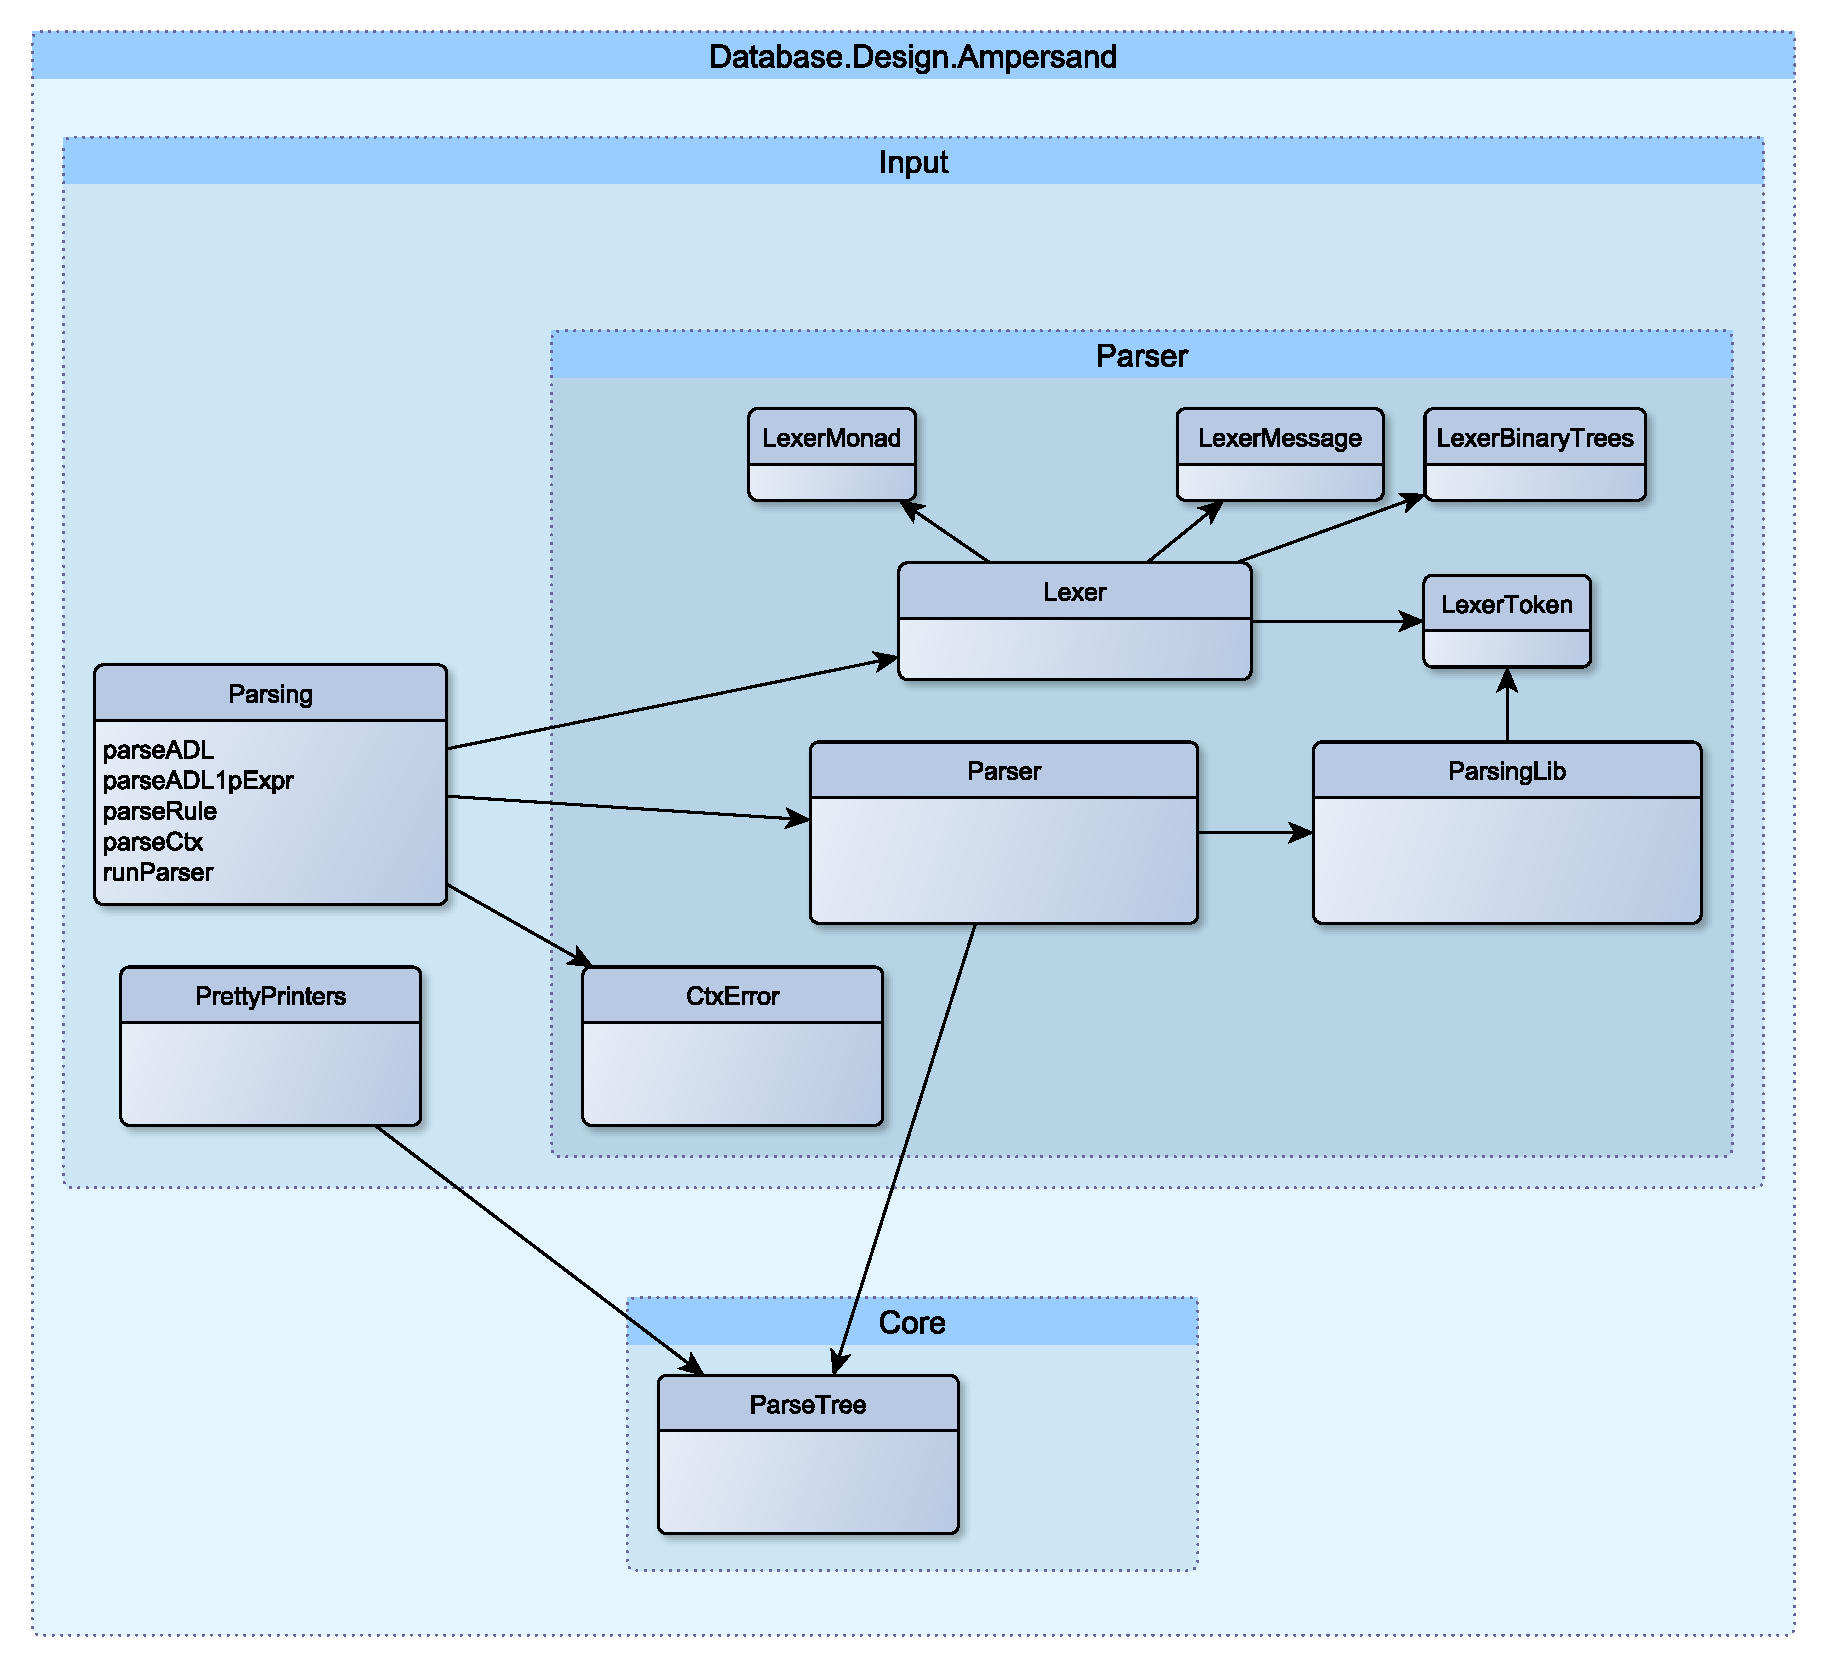
\includegraphics[width=\columnwidth]{Figures/ParserModules}
    \caption{The parser modules and their relationships}
    \label{fig:ParserModules}
  \end{figure}%
  TODO: Add the exported functions to each module.

  \subsubsection{Modules}
  \label{subsec:parser-modules}
  In this section a short description of each module is given:
  %
  \begin{description}
    \item[Parsing] module that implements the interface of the parser with the rest of the system.
      It is responsible for reading the input files, calling the lexer and the parser and returning a parse tree as result (or a parse error).

    \item[Parser] module responsible for executing the parsing itself.
      It accepts the tokens that are allowed in each grammar production and generates the corresponding parse tree.
      The parser is described in \autoref{subsec:design-parser}.
      
    \item[ParsingLib] library that contains several useful functions to assist the parser, e.g. token recognition.
      These functions are not depending on the specific grammar rules.
      
    \item[ParseTree] external module containing the parse tree data structures.
      Only details of this module have been changed during this project (e.g. field ordering).
    
    \item[PrettyPrinters] contains the \texttt{Pretty} class and the functions responsible for printing the parse tree to ADL scripts in a `pretty' way.
    
    \item[CtxError] contains the data structures responsible for the parse errors and their location.
      This module has not been refactored as a part of this project.
    
    \item[Lexer] module responsible for recognizing the input characters and converting them to tokens.
      The lexer is described in \autoref{subsec:lexer}.
    
    \item[LexerMonad] contains a monad definition that supports lexing with context.
      It tracks for example the location in the input and the warnings that may be generated.
    
    \item[LexerMessage] contains functions to handle errors and warnings from the lexer.
    
    \item[LexerBinaryTrees] module responsible for searching binary trees in an efficient way, to support the token recognition.
    
    \item[LexerToken] contains the data structure that represents the input tokens for the lexer.
      The tokens work as an interface between the lexer and the parsing library.
  \end{description}

\subsection{Changes due to Parsec (D)}
TODO: Show the differences between uulib and Parsec, e.g. the try for backtracking.

\subsection{Lexer (M)}
\label{subsec:lexer}
TODO: describe how the lexer works, and the improvements done to it.

\subsection{Parser (D)}
\label{subsec:design-parser}
TODO: describe how the parser is implemented.

\subsubsection{Parsing library (D)}
\label{subsec:design-parsing-lib}
TODO: reference the phase 3a decision to use parsec.

\subsubsection{Backtracking (D)}
TODO: describe why the try-statements are necessary.

\subsection{Parse tree (R-M)}
\label{subsec:design-parse-tree}
Improvements in the Ampersand parse tree are out of the scope of this project, because of the potential consequences to the rest of the Ampersand system.
However, during the development of the new parser a few constructions have been changed in order to make the parser more readable and maintainable.
The changes have been mostly in the order of the constructor parameters, and this was done consequently though all Ampersand modules.
The updated parse tree is depicted in the appendices (\autoref{fig:parse-tree}).

\subsection{Errors (M)}
TODO: show what we've done to improve the errors.

\subsection{Next steps (M)}
TODO: give tips on how to further improve the parser. e.g.:
  - cleanup CtxError, add warnings, use <?> for the errors.
  - reorganize parse tree, e.g. using always Origin as first parameter.